\documentclass[twoside]{article}
\usepackage{amssymb}
\usepackage{amsthm}
\usepackage{amsmath}
\usepackage{amsfonts}
\usepackage[utf8]{inputenc}
\usepackage[spanish]{babel}
\usepackage{tikz}
\usepackage{centernot}
\usepackage{hyperref}
\usepackage{fancyhdr}
\usepackage{lipsum}
\usepackage{subcaption}
\hypersetup{
    colorlinks,
    citecolor=black,
    filecolor=black,
    linkcolor=black,
    urlcolor=black
}
\usepackage{xurl}
\usepackage[top=1in, bottom=1.5in, left=1in, right=1in]{geometry}
\pagestyle{fancy}
\fancyhead{}
\fancyhead[L]{\leftmark}
\fancyfoot{}
\fancyfoot[C]{\thepage}
\newcommand{\enquote}[1]{``#1''}
\usepackage{float}
\usepackage[parfill]{parskip}
\newcommand{\image}[2]{
\begin{figure}[H]
    \includegraphics[width=#1 cm]{../images/#2.png}
    \centering
\end{figure}
}

\title{Práctica 4 SWAP}
\author{XuSheng Zheng}
\date{}

\begin{document}

\maketitle
\tableofcontents
\newpage

\section{Certificado autoafirmado SSL}
Empezamos habilitando el módulo SSL de Apache y creando el directorio para ubicar los certificados:
\image{8}{1}
Ahora creamos los certificados con los siguientes datos:
\image{8}{2}
\subsection{Opciones avanzadas}
De las opciones introducidas anteriormente, podemos prescindir de \textbf{nodes} para añadir una contraseña a la clave. Además, tenemos las siguientes opciones que pueden ser interesantes:
\begin{itemize}
    \item \textbf{-config filename}: permite especificar un archivo de configuración para la creación de los certificados.
    \item \textbf{-subj arg}: permite especificar datos para la creación del certificado. El argumento debe ser de la forma \textbf{/type0=value0/type1=value1/type2=....}. Al introducir esta opción no nos pedirá los datos como habíamos hecho.
    \item \textbf{-addext ext}: permite añadir una extensión de x509 en el certificado generado.
\end{itemize}
Como ejemplo creamos el siguiente certificado:
\image{8}{5}
Podemos ver que nos pide la contraseña para generar los certificados. Si eliminamos la opción \textbf{-subj} podemos ver que aparte de pedirnos la contraseña nos pide también el resto de informaciones:
\image{8}{6}

\section{Apache con certificado SSL}
Editamos el archivo de configuración \textit{/etc/apache2/sites-available/default-ssl.conf}:
\image{8}{3}
Activamos \textbf{default-ssl} y reiniciamos Apache:
\image{8}{4}
Para comprobar que se ha instalado correctamente el certificado accedemos desde el navegador del anfitrión:
\image{12}{8}
Accedemos al certificado desde el candado con exclamación a la izquierda de la URL:
\image{8}{9}
\image{12}{7}



\begin{figure}[H]
    \centering
    \begin{subfigure}{.5\textwidth}
        \centering
%        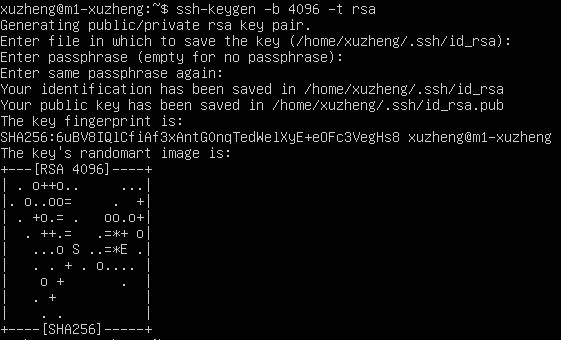
\includegraphics[width=7cm]{../images/13.png}
    \end{subfigure}%
    \begin{subfigure}{.5\textwidth}
        \centering
%        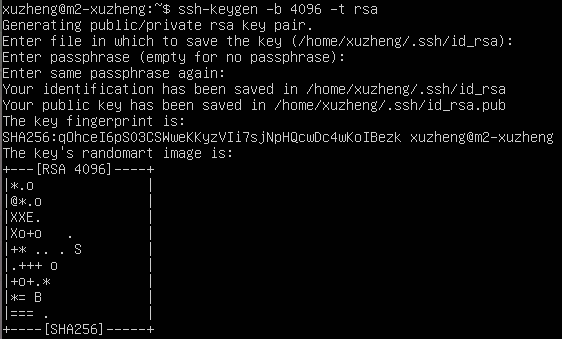
\includegraphics[width=7cm]{../images/14.png}
    \end{subfigure}
\end{figure}


\newpage
\section{Bibliografía}
\begin{itemize}
    \item \url{https://linux.die.net/man/1/scp}
    \item \url{https://linux.die.net/man/1/tar}
    \item \url{https://serverfault.com/questions/141773/what-is-archive-mode-in-rsync}
    \item \url{https://ss64.com/bash/rsync.html}
    \item \url{https://linux.die.net/man/1/rsync}
    \item \url{https://serverfault.com/questions/123629/run-task-every-90-minutes-with-cron}
\end{itemize}

\end{document}
